% background
% brief review of previous research (cite)
% reson why the research was undertaken
% Hypothesis
% explenation of techniques and why they ve been chosen
% objectives = what you hope to achieve
% brief reference to the main outcome

%$\ce{CdS_x Se_{1-x}/ZnS}$



\section{Introduction}
\label{sec:Introduction}

As the resistivity of metals and semiconductors depends on the temperature in different ways,
here a temperature dependent resistance measurement is done in order to characterize the samples of 
(1)germanium, (2)copper and (3)nickel, where the germanium represents a semiconductor.

The resistance $R$ can be measured as a voltage drop $V$ over a sample with current $I$.
The aim of a resistivity ($\rho$) measurement is to derive the resistivity of the material, which is defined as the reciprocal of the conductivity

\begin{equation}
    \sigma = 1 / \rho = J / E = q n \mu,
\end{equation}
where $J$ is the current density and $E$ the electric field intensity.
Further, $q$ is the elemtary charge, $\mu$ the charge carrier mobility and $n$ the carrier density.#
Here, the macroscopic definition is based on a microscopic model for carrier mobility.
Another definition of the resistivity for uniform samples is given by 
\begin{equation}
    \rho = R S / L,
\end{equation}
where L is the length of the sample and S its cross-section.

\subsection{Experimental sutup}
\label{sec:setup}

\begin{figure*}
  \centering
  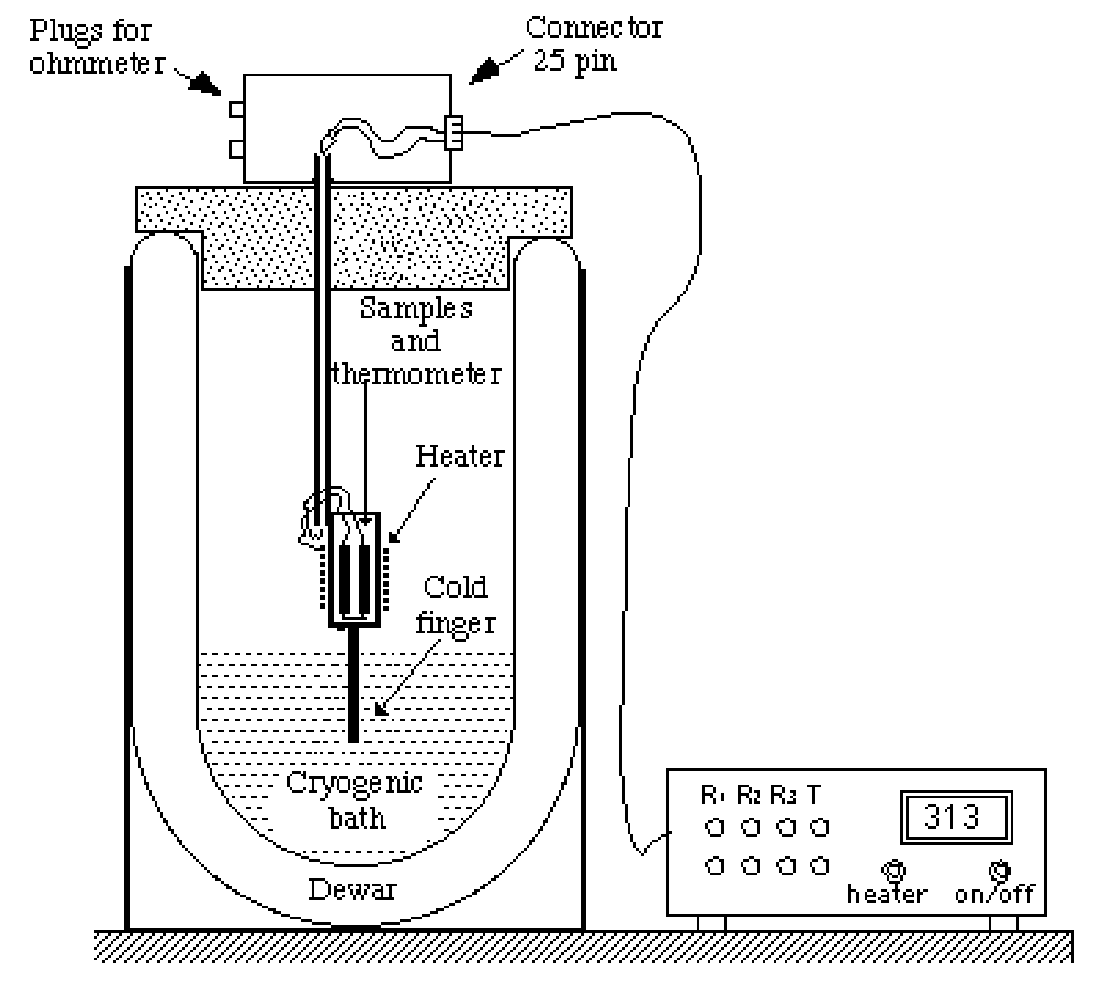
\includegraphics[width=0.55\textwidth]{graphics/setup.png}
  \caption[width=0.4\textwidth]{Schematic setup of the experiment\cite{instruction}.}
  \label{fig:setup}
\end{figure*}

The apperatus includes three samples, and allows time resolved, temperature dependend resistance measurements.
As depicted schematically in figure \ref{ig:setup}, the samples are inside a brass sampleholder which can be cooled down by brining the cold finger in contact with liquid nitrogen.
Therefore, the whole apperatus is positioned into a dewar.
A $\SI{50}{\ohm}$ heater is installed inside the sampleholder to reach temperatures up to $\SI{450}{\degree\celsius}$.

The samples are wired inside the sampleholder and connected to a controlunit.
Also a thermometer is installed to overlook the current sample temperature.

The controlunit is providing power supply to the heater, the samples current bias and to the therometer.

In technical detail, the absolute temperature T is measured by the forward voltage of a PN junction on constant current bias. 
The samples resistance measurement is done by using a four wires volt-amperometric architecture mentioned in chapter \ref{sec:R-measurement}. 
Here, in order to eliminate the effect of wire amd contact resistance, the current supply is separated by the voltage measurement by using 4 wires instead of two.

The metalic samples are thin wires with a nominal diameter of $\SI{0.05}{\milli\meter}$ and a few centimeters long, whereas the germanium sample is a $\SI{1}{\milli\meter}$ thick wafer, cut into a $\SI{3}{\milli\meter} \times \SI{5}{\milli\meter}$ plate.
The bias currents are $\SI{1}{\milli\Ampere}$ for germanium, $\SI{2}{\milli\Ampere}$ for nickel and $\SI{10}{\milli\Ampere}$ for copper.

To amplify the differential voltage signal along the sample a high input impedance operational amplifier (INA114) with sample dependant gain G is used.
The choosen values are $G_1 = 100,G_2=10 and G_3=1$, which is reciprocal to the sensitivity of the output voltage measurement.
The temperature channel has a sensitivity of $\SI{10}{\milli\volt\per\kelvin}$ in the temperature range of the experiment.

To use the LoggerProaquisition program on the PC, the LabPro surface is used. 
The Aquisition module is connected by a standard 25-pin cable to the PC.

The samples are also connected to four banana plugs, where they are called S1,S2,S3 and GND.
Therefore, it is possible to measue the resisance by the two wires technique mentioned in chapter \ref{sec:R-measurement}.
Also a four wires resistance measurement, as elaborated in chapter \ref{sec:R-measurement} can be done.

\subsection{Resistivity measurement circuits}
\label{sec:R-measurement}

\begin{figure*}
    \centering
    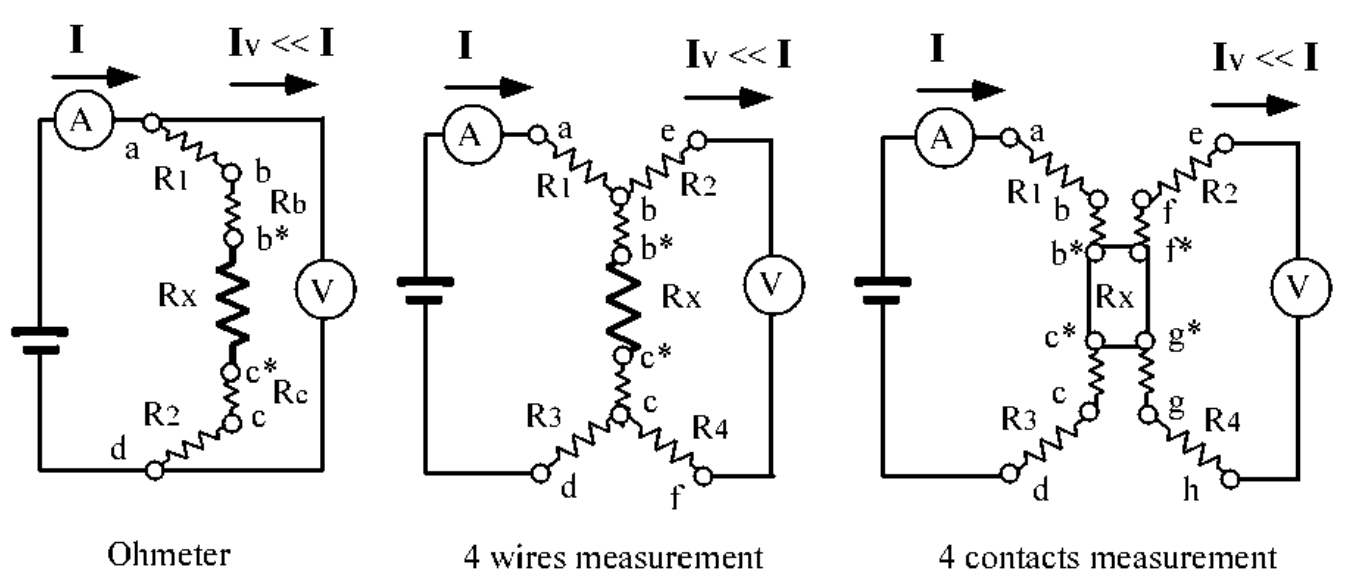
\includegraphics[width=0.7\textwidth]{graphics/r-measure.png}
    \caption[width=0.7\textwidth]{Schematic setup of the experiment\cite{instruction}.}
    \label{fig:setup}
  \end{figure*}